\chapter{ Guía de Usuario}
\label{chap:manual-usuario}

RobotUI es una aplicación web creada con un claro propósito; el de  proporcionar a los usuarios un medio donde compartir sus dispositivos robóticos con el resto de usuarios.\\

Para ello RobotUI proporciona una serie de herramientas para que, aquellas personas que no tengan los suficientes conocimientos de programación, puedan configurar un
entorno para el manejo de sus proyectos robóticos y tener posibilidad de compartir sus experiencias con el resto.\\

La particularidad de RobotUI es que el usuario propietario del robot tiene la posibilidad de permitir el manejo de sus dispositivos robóticos al resto de usuarios que él mismo considere de una 
manera controlada además de él mismo o, por otra parte, permitir que otros usuarios visualicen, como si de espectadores se tratase, el control que un determinado usuario realiza de un determinado robot.
Todo ello en tiempo real.\\

Por tanto, tras esta breve introducción en el ámbito de la aplicación, en este manual se describen los diferentes paso a realizar para configurar sus dispositivos correctamente en el sistema
y abrirlo a toda una comunidad de usuarios. Además de tener abierto el acceso a otros muchos dispositivos de otros usuarios.\\

\subsection{Objetivo de esta guía}

Esta guía tiene como objetivo la de proporcionar al usuario un soporte de ayuda e
iniciación a la utilización de RobotUI.\\

Esta sección comprende:\\

\begin{itemize}
 \item Guía de acceso al código fuente de la aplicación.
 \item Guía de uso de la aplicación.
 \item Guía para la puesta en marcha y programación de un robot.
\end{itemize}

\subsection{Dirigido a}

Esta guía esta dirigida al usuario final del proyecto RobotUI. Tiene la finalidad de proporcionar una guía descriptiva de los procedimientos de creación, configuración y utilización de los diferentes dispositivos 
en sus dos modalidades disponibles, la de control y la de visualización.

\subsection{Obtener RobotUI}

El código fuente junto con la presente memoria se encuentra disponible en el repositorio GitHub en el enlace \url{https://github.com/lopi87/SAILS-RobotUI} o usando la herramienta
Git, escribiendo en la consola el siguiente comando:\\

\begin{lstlisting}[language=bash]
 git clone git@github.com:lopi87/SAILS-RobotUI.git 
\end{lstlisting}


\section{ Uso de RobotUI }
\label{sec:uso-robotui}


\begin{figure}[H]
  \begin{center}
    
\includegraphics[scale=0.5]{imagenes/manual-usuario/barra-menu1.png}
  \end{center}
  \caption{Página principal RobotUI.}
  \label{website:pagina-principal}
\end{figure}

\begin{figure}[H]
  \begin{center}
    
\includegraphics[scale=0.5]{imagenes/manual-usuario/barra-menu2.png}
  \end{center}
  \caption{Página principal RobotUI.}
  \label{website:pagina-principal}
\end{figure}




\subsection{ Registo de usuario }
\label{sec:creacion-usuario}

\begin{figure}[H]
  \begin{center}
    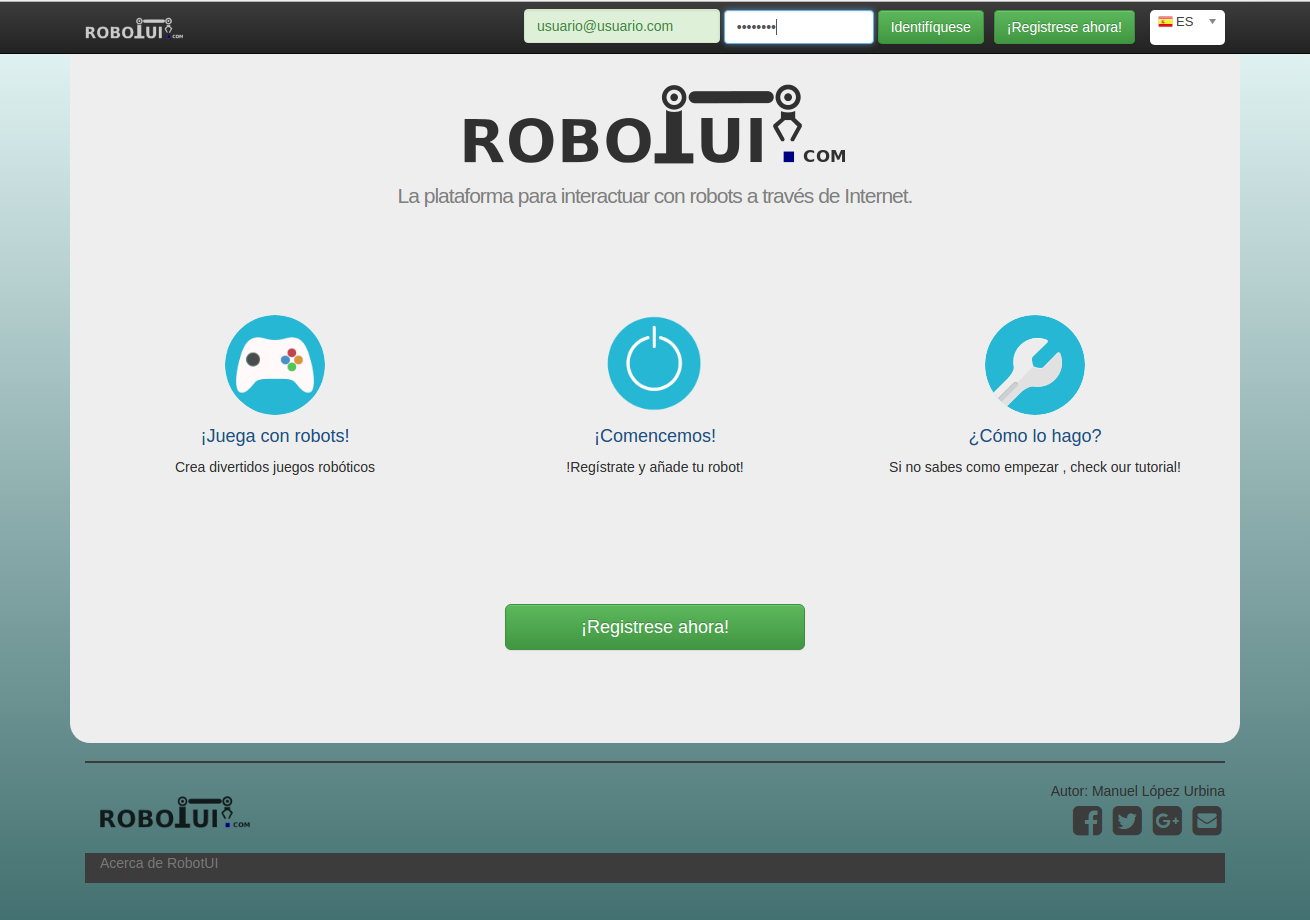
\includegraphics[scale=0.3]{imagenes/manual-usuario/pagina-principal.png}
  \end{center}
  \caption{Página principal RobotUI.}
  \label{website:pagina-principal}
\end{figure}

\subsection{Creación de un Robot}
\label{sec:creacion-robot}

Para el proceso de creación de un robot hacemos click al menú \emph{Robots} \textrightarrow \enspace \emph{Mis robots} accediendo al formulario de creación.

En este caso registraremos nuestro robot de pruebas descrito en el capítulo \label{cap:robot}. Para ello introducimos los siguientes datos:

\begin{enumerate}
 \item Nombre: nombre de nuestro robot.
 \item Dirección IP: dirección donde se encontrará accesible nuestro robot.
 \item Puerto: puerto donde se encontrará nuestro robot a la escucha de conexiones.
 \item Descripción: campo opcional en el que podemos añadir una descripción de nuestro robot y que será visible al resto de usuarios.
 \item Imagen: campo opcional en el que podremos subir una imagen de nuestro robot.
 \item Usuarios espectadores: selector en el que podemos especificar qué usuarios del sistema tendrán permisos para visualizar el funcionamiento de nuestro robot.
 \item Usuarios controladores: selector para especificar qué usuarios podrán tomar control de nuestro robot.
 \item Público: checkboxes para indicar si por el contrario, el robot que abierto a todos los usuarios para su control o abierto para su visualización si marcamos el primero o el segundo checkbox respectivamente
 y haciendo por tanto inválidos los parámetros de los slectores anteriores.
\end{enumerate}

Una vez rellenado los campos como se muestran en la imagen \label{website:creacion-robot} pulsamos en \icontext{.2}{.35}{imagenes/manual-usuario/btn-crear.png}.

\begin{figure}[H]
  \begin{center}
    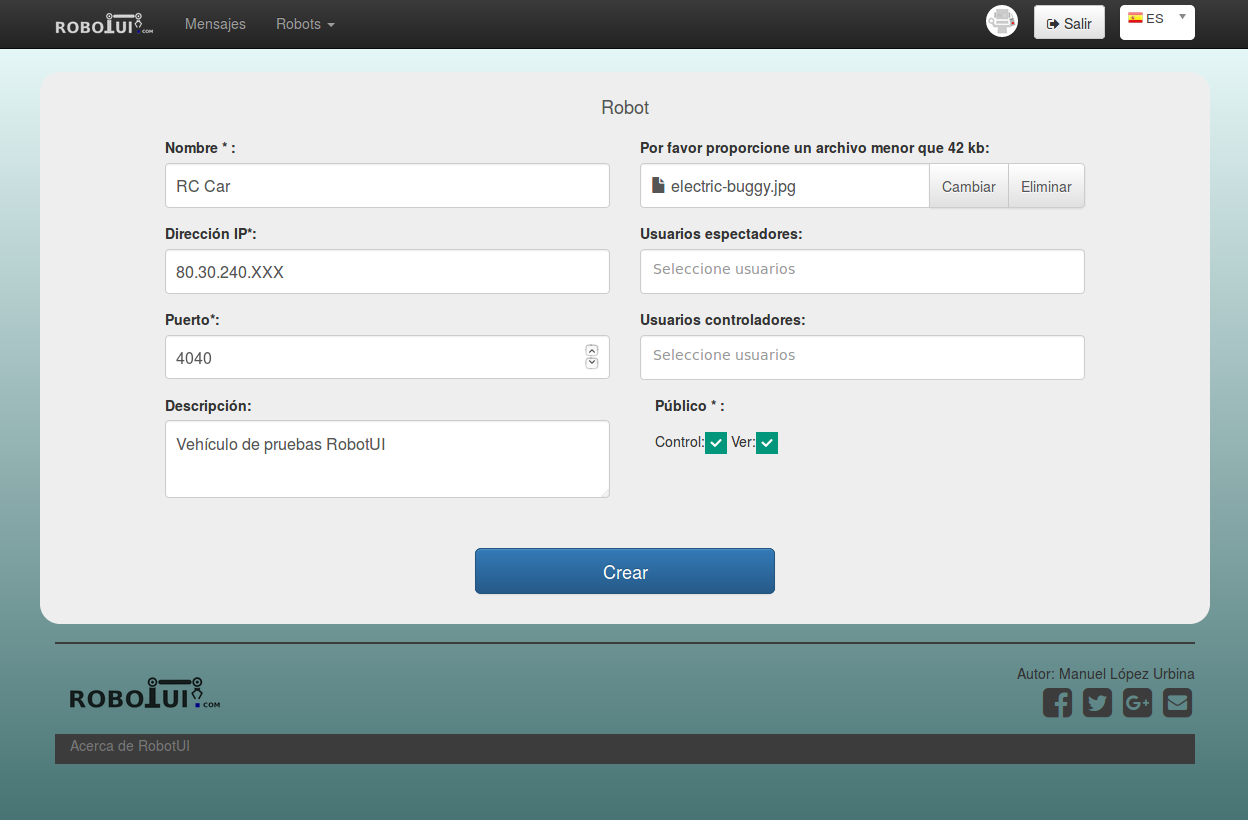
\includegraphics[scale=0.3]{imagenes/manual-usuario/pagina-crear-robot.png}
  \end{center}
  \caption{Formulario de creación de un robot.}
  \label{website:creacion-robot}
\end{figure}



\subsection{Configuración de la interfaz}

Una vez creado nuestro robot en el sistema ya podemos configurar su interfaz. En la figura \ref{website:Configuracion-interfaz} podemos ver el canvas sobre el que iremos añadiendo los diferentes elementos que 
conformarán nuestro panel de control.

\begin{figure}[H]
  \begin{center}
    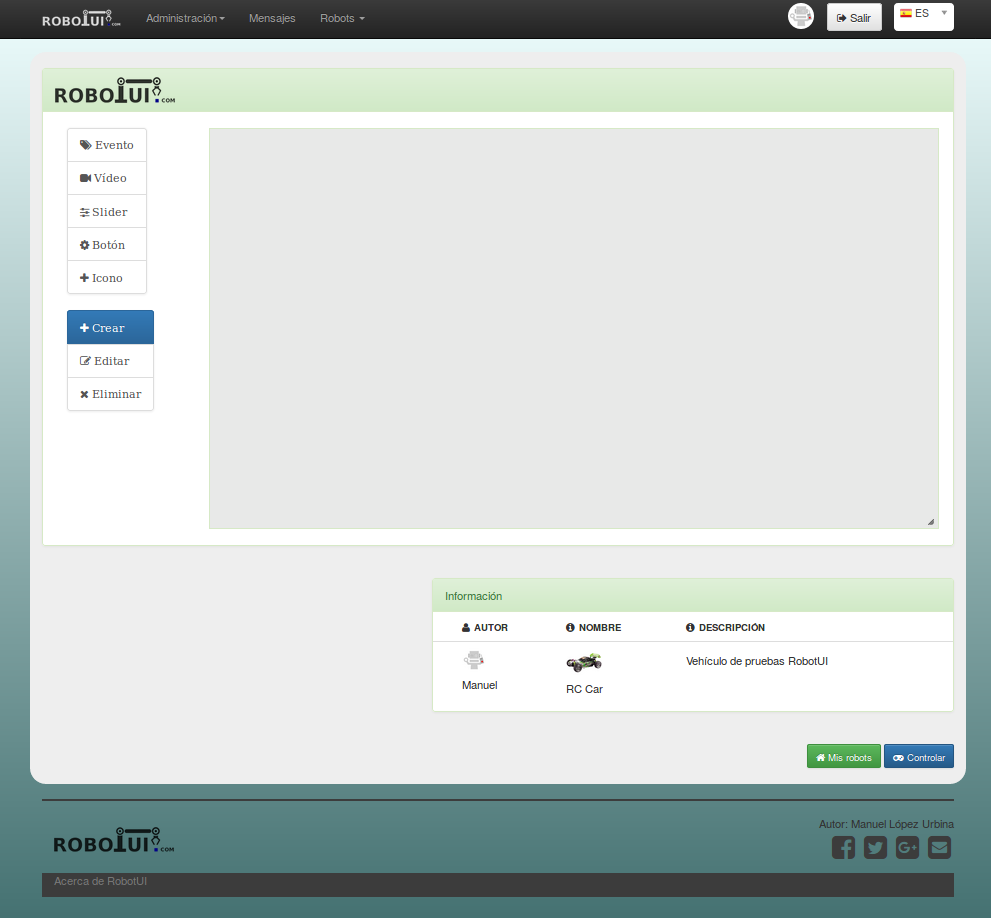
\includegraphics[scale=0.4]{imagenes/manual-usuario/pagina-configurar-interfaz.png}
  \end{center}
  \caption{Panel de configuración de la interfaz.}
  \label{website:Configuracion-interfaz}
\end{figure}



\begin{figure}[H]
  \begin{center}
    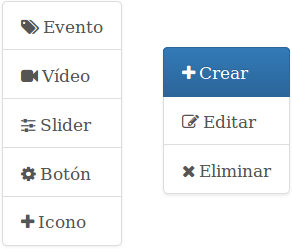
\includegraphics[scale=.6]{imagenes/manual-usuario/barra-herramientas-interfaz.png}
  \end{center}
  \caption{Panel de herramientas  y panel de acciones para la configuración de la interfaz.}
  \label{website:pagina-principal}
\end{figure}


\begin{table}[H]
  \begin{center}
    \begin{tabular}{|p{2cm}|p{10cm}|}
      \hline
      \centering{Botón} & \qquad \quad Significado \\
      \hline
      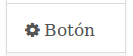
\includegraphics[width=2cm]{imagenes/manual-usuario/nuevo-boton.png} & Apertura del formulario para la creación de un botón. \\
      \hline
    \end{tabular}
  \end{center}
\caption{Elementos de una interfaz.}
\end{table}


\section{ Programa tu robot }
\label{sec:programacion-robot}


